\section{Introdução}

O problema de encontrar o menor caminho (\emph{All pairs shortest path}) é aquele em que
buscamos o menor caminho entro quaisquer dois pares de nós em grafo direcionado. A
\cref{fig:grafo-input6} exemplifica o tipo de grafo que tratamos e a matriz que
usamos para representar este mesmo grafo, onde cada entrada \(M_{ij}\) é a distância
da aresta que vai do nó \(i\) ao nó \(j\).

\begin{figure}[htp]
	\centering
	\begin{minipage}{.4\linewidth}
		\centering
		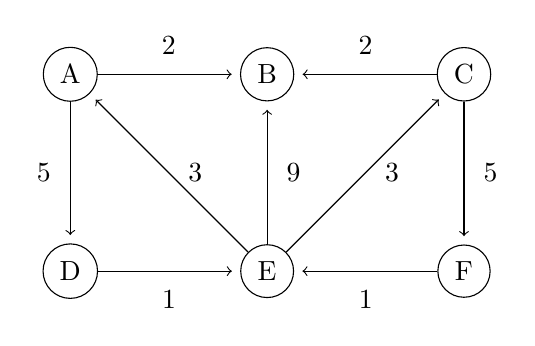
\begin{tikzpicture}[
				every path/.style = {->, shorten >= 3pt},
				every node /.style = {draw, circle, node distance = 6cm, inner sep = 3pt, minimum width = 3cm}
			]

			\node (a) [circle, draw] {A};
			\node (b) [right of = a, node distance = 2.5cm, circle, draw] {B};
			\node (c) [right of = b, node distance = 2.5cm, circle, draw] {C};
			\node (d) [below of = a, node distance = 2.5cm, circle, draw] {D};
			\node (e) [right of = d, node distance = 2.5cm, circle, draw] {E};
			\node (f) [right of = e, node distance = 2.5cm, circle, draw] {F};

			\path
			(a) edge node [label=above:{2}] {} (b)
			(a) edge node [label=left:{5}] {} (d)
			(c) edge node [label=above:{2}] {} (b)
			(c) edge node [label=right:{5}] {} (f)
			(d) edge node [label=below:{1}] {} (e)
			(e) edge node [label=right:{3}] {} (a)
			(e) edge node [label=right:{9}] {} (b)
			(e) edge node [label=right:{3}] {} (c)
			(f) edge node [label=below:{1}] {} (e);
		\end{tikzpicture}
	\end{minipage}
	\begin{minipage}{.4\linewidth}
		\centering
		\begin{equation*}
      M = 
			\begin{bmatrix}
				0 & 2 & 0 & 5 & 0 & 0 \\
				0 & 0 & 0 & 0 & 0 & 0 \\
				0 & 2 & 0 & 0 & 0 & 5 \\
				0 & 0 & 0 & 0 & 1 & 0 \\
				3 & 9 & 3 & 0 & 0 & 0 \\
				0 & 0 & 0 & 0 & 1 & 0
			\end{bmatrix}
		\end{equation*}
	\end{minipage}
	\caption{Grafo direcionado com valores atribuídos para cada aresta e a matriz quadrada correspondente.}%
	\label{fig:grafo-input6}
\end{figure}

A solução deste problema é também uma matriz quadrada, onde cada entrada \(N_{ij}\) é o disância do menor caminho
possível a ser percorrida para ir do nó \(i\) ao \(j\).

\[N = 
\begin{bmatrix}
	0 & 2 & 9 & 5  & 6 & 14 \\
	0 & 0 & 0 & 0  & 0 & 0  \\
	9 & 2 & 0 & 14 & 6 & 5  \\
	4 & 6 & 4 & 0  & 1 & 9  \\
	3 & 5 & 3 & 8  & 0 & 8  \\
	4 & 6 & 4 & 9  & 1 & 0
\end{bmatrix}
\]

Neste trabalho, iremos descrever uma solução para este problema adotando paralelismo através de \ac{mpi} usando
o \emph{algoritmo de Fox}, distribuindo processos entre diversas configurações de máquinas e os organizando 
em um comunicador de \emph{grid}.
